\documentclass{beamer}
%\usepackage[utf8]{inputenc}
%\usetheme{Warsaw}
\usetheme{boadilla}
%\usetheme{default}
\usecolortheme{beaver}

\usepackage[utf8]{inputenc} 
\usepackage[T1]{fontenc}
\usepackage[upright]{fourier} 
%\usepackage[usenames,dvipsnames]{xcolor}
\usepackage{tkz-kiviat,numprint} 
\usetikzlibrary{arrows}
\usepackage{pgfplots}
%\usepackage{tikz}
%\usepackage[francais]{babel}
%\usepgfplotslibrary{external}
% 
%\tikzexternalize 

\pgfplotsset{width=7cm,	compat=1.12}

%%-------------------------------------------------------------------------------
%          -Packages nécessaires pour écrire en Français et en UTF8-
%-------------------------------------------------------------------------------
\usepackage[utf8]{inputenc}
\usepackage[frenchb]{babel}
\usepackage[T1]{fontenc}
\usepackage{lmodern}
\usepackage{textcomp}

%-------------------------------------------------------------------------------

%-------------------------------------------------------------------------------
%                          -Outils de mise en forme-
%-------------------------------------------------------------------------------
\usepackage{hyperref}
\hypersetup{pdfstartview=XYZ}
\usepackage{enumerate}
\usepackage{graphicx}
%\usepackage{multicol}
%\usepackage{tabularx}

%\usepackage{anysize} %%pour pouvoir mettre les marges qu'on veut
%\marginsize{2.5cm}{2.5cm}{2.5cm}{2.5cm}

\usepackage{indentfirst} %%pour que les premier paragraphes soient aussi indentés
\usepackage{verbatim}
%\usepackage[table]{xcolor}  
%\usepackage{multirow}
\usepackage{ulem}
%-------------------------------------------------------------------------------


%-------------------------------------------------------------------------------
%                  -Nécessaires pour écrire des mathématiques-
%-------------------------------------------------------------------------------
\usepackage{amsfonts}
\usepackage{amssymb}
\usepackage{amsmath}
\usepackage{amsthm}
\usepackage{tikz}
\usepackage{xlop}
\usepackage[output-decimal-marker={,}]{siunitx}
%-------------------------------------------------------------------------------


%-------------------------------------------------------------------------------
%                    - Mise en forme 
%-------------------------------------------------------------------------------

\newcommand{\bu}[1]{\underline{\textbf{#1}}}


\usepackage{ifthen}


\newcommand{\ifTrue}[2]{\ifthenelse{\equal{#1}{true}}{#2}{$\qquad \qquad$}}

\newcommand{\kword}[1]{\textcolor{red}{\underline{#1}}}


%-------------------------------------------------------------------------------



%-------------------------------------------------------------------------------
%                    - Racourcis d'écriture -
%-------------------------------------------------------------------------------

% Angles orientés (couples de vecteurs)
\newcommand{\aopp}[2]{(\vec{#1}, \vec{#2})} %Les deuc vecteurs sont positifs
\newcommand{\aopn}[2]{(\vec{#1}, -\vec{#2})} %Le second vecteur est négatif
\newcommand{\aonp}[2]{(-\vec{#1}, \vec{#2})} %Le premier vecteur est négatif
\newcommand{\aonn}[2]{(-\vec{#1}, -\vec{#2})} %Les deux vecteurs sont négatifs

%Ensembles mathématiques
\newcommand{\naturels}{\mathbb{N}} %Nombres naturels
\newcommand{\relatifs}{\mathbb{Z}} %Nombres relatifs
\newcommand{\rationnels}{\mathbb{Q}} %Nombres rationnels
\newcommand{\reels}{\mathbb{R}} %Nombres réels
\newcommand{\complexes}{\mathbb{C}} %Nombres complexes


%Intégration des parenthèses aux cosinus
\newcommand{\cosP}[1]{\cos\left(#1\right)}
\newcommand{\sinP}[1]{\sin\left(#1\right)}

%Fractions
\newcommand{\myfrac}[2]{{\LARGE $\frac{#1}{#2}$}}

%Vocabulaire courrant
\newcommand{\cad}{c'est-à-dire}

%Droites
\newcommand{\dte}[1]{droite $(#1)$}
\newcommand{\fig}[1]{figure $#1$}
\newcommand{\sym}{symétrique}
\newcommand{\syms}{symétriques}
\newcommand{\asym}{axe de symétrie}
\newcommand{\asyms}{axes de symétrie}
\newcommand{\seg}[1]{$[#1]$}
\newcommand{\monAngle}[1]{$\widehat{#1}$}
\newcommand{\bissec}{bissectrice}
\newcommand{\mediat}{médiatrice}
\newcommand{\ddte}[1]{$[#1)$}

%Figures
\newcommand{\para}{parallélogramme}
\newcommand{\paras}{parallélogrammes}
\newcommand{\myquad}{quadrilatère}
\newcommand{\myquads}{quadrilatères}
\newcommand{\co}{côtés opposés}
\newcommand{\diag}{diagonale}
\newcommand{\diags}{diagonales}
\newcommand{\supp}{supplémentaires}
\newcommand{\car}{carré}
\newcommand{\cars}{carrés}
\newcommand{\rect}{rectangle}
\newcommand{\rects}{rectangles}
\newcommand{\los}{losange}
\newcommand{\loss}{losanges}


%----------------------------------------------------

\title{Conseil de Classe 3e}
\author{}\institute[GS. S$^t$ Vincent, S$^t$ Bernard]{Groupe Scolaire S$^t$ Vincent, S$^t$ Bernard}


%\AtBeginSubsection[]
%{
%	\begin{frame}
%		\frametitle{}
%		\tableofcontents[currentsection, currentsubsection]
%	\end{frame} 
%}

\begin{document}
	
	
	
\begin{frame}
	\titlepage
\end{frame}


\begin{frame}


\begin{tikzpicture}
\begin{axis}[
	ytick={0,2,...,20},
	minor y tick num={0},
	ybar,
	bar width= 6pt,
	%enlargelimits=0.15,
	legend style={at={(0.5,-0.15)},
			anchor=north, legend columns=-1},
	ylabel={Moyenne},
	symbolic x coords={{maths}, {histoire}, {EPS}, {anglais}, {techno}},
	xtick=data,
	nodes near coords,
	every node near coord/.append style={font=\tiny},
	nodes near coords align={vertical},
	width=.8\textwidth,
	]
	
\addplot[ybar,fill=blue] coordinates {
	(maths,15)
	(histoire,18)
	(EPS,12.5)
	(anglais,15)
	(techno, 13)
	
};

\addplot[ybar,fill=red] coordinates {
	(maths,17)
	(histoire,15)
	(EPS,9.5)
	(anglais,10.5)
	(techno, 12)
};

\addplot[ybar,fill=green] coordinates {
	(maths,15)
	(histoire,17)
	(EPS,11)
	(anglais,12.5)
	(techno, 14)
};

\legend{1er tri, 2e tri, 3e tri}
\end{axis}
\end{tikzpicture}	
	

\end{frame}

\begin{frame}
\frametitle{ACAR Omer (18/12/2000)}  
\framesubtitle{ }	


\begin{columns}[onlytextwidth]



\begin{column}{0.3\textwidth}
	\vspace*{.5cm}
	\begin{center}
			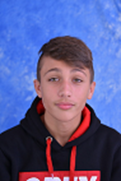
\includegraphics[scale=0.8]{tof}
	\end{center}

	
	\begin{block}{Métier envisagé}
		Assureur
	\end{block}
	
	\begin{alertblock}{Orientation}
		\begin{enumerate}
			\item 2$^{de}$ GT
			\item BAC PRO COM
		\end{enumerate}
	\end{alertblock}
	
	
\end{column}	

\begin{column}{0.70\textwidth}
	
		\begin{center}
		
		\vspace*{-.7cm}	

		{\small \begin{tabular}{cccc}
			& Classe                       & \'Elève                      & Classement                   \\
			{\color[HTML]{00009B} Trimestre 1} & {\color[HTML]{00009B} 12,40} & {\color[HTML]{00009B} 10.52} & {\color[HTML]{00009B} 22/27} \\ \hline
			{\color[HTML]{FE0000} Trimestre 2} & {\color[HTML]{FE0000} 11,69} & {\color[HTML]{FE0000} 10.11} & {\color[HTML]{FE0000} 25/28} \\ \hline
			{\color[HTML]{34FF34} Trimestre 3} & {\color[HTML]{34FF34} 12,46} & {\color[HTML]{34FF34} 11.69} & {\color[HTML]{34FF34} 16/29}
		\end{tabular}}
		
	

{\color{blue} Moyenne élève}
{\color{red} Moyenne classe}

\vspace*{-0.8cm}



\begin{tikzpicture}[label distance=.15cm,rotate=30,scale=.45]
\tkzKiviatDiagram[radial=7,lattice=4,gap=1,step=0.2,label space=1.2]%
{Maths,
	Histoire Géo,
	Français,
	EPS,
	SVT,
	Techno,
	Physique}
\tkzKiviatLine[thick,color=red,fill=red,opacity=.15](12,15,14,11,13,10, 15)
\tkzKiviatLine[thick,color=blue](15,16,13,18,11,7, 18)
\tkzKiviatGrad[prefix=,unity=5](0)   
\end{tikzpicture}

	\end{center}
	
\end{column}	

\end{columns}

\end{frame}




\begin{frame}
	\frametitle{CHOPPARD Justine (18/12/2000)}  
	\framesubtitle{ }	
	
	
	\begin{columns}[onlytextwidth]
		
		
		
		\begin{column}{0.3\textwidth}
			\vspace*{-.5cm}
			\begin{center}
				\includegraphics[scale=0.7]{tof2}
			\end{center}
			
			
			\begin{block}{Métier envisagé}
				Anesthésiste
			\end{block}
			
			\begin{alertblock}{Orientation}
				\begin{enumerate}
					\item 2$^{de}$ GT
				\end{enumerate}
			\end{alertblock}
			
			
		\end{column}	
		
	\begin{column}{0.70\textwidth}
		
		\begin{center}
			
			\vspace*{-.7cm}	
			
			{\small \begin{tabular}{cccc}
					& Classe                       & \'Elève                      & Classement                   \\
					{\color[HTML]{00009B} Trimestre 1} & {\color[HTML]{00009B} 12,40} & {\color[HTML]{00009B} 10.52} & {\color[HTML]{00009B} 22/27} \\
					{\color[HTML]{FE0000} Trimestre 2} & {\color[HTML]{FE0000} 11,69} & {\color[HTML]{FE0000} 10.11} & {\color[HTML]{FE0000} 25/28} \\
					{\color[HTML]{34FF34} Trimestre 3} & {\color[HTML]{34FF34} 12,46} & {\color[HTML]{34FF34} 11.69} & {\color[HTML]{34FF34} 16/29}
				\end{tabular}}
				
				
				
				{\color{blue} Moyenne élève}
				{\color{red} Moyenne classe}
				
				\vspace*{-0.8cm}
				
				
				
				\begin{tikzpicture}[label distance=.15cm,rotate=30,scale=.45]
				\tkzKiviatDiagram[radial=7,lattice=4,gap=1,step=0.2,label space=1.2]%
				{Maths,
					Histoire Géo,
					Français,
					EPS,
					SVT,
					Techno,
					Physique}
				\tkzKiviatLine[thick,color=red,fill=red,opacity=.15](12,15,14,11,13,10, 15)
				\tkzKiviatLine[thick,color=blue](18,17,19,18.5,19,17, 18)
				\tkzKiviatGrad[prefix=,unity=5](0)   
				\end{tikzpicture}
				
			\end{center}
			
		\end{column}
			
		\end{columns}
		
	\end{frame}




\end{document}


\begin{frame}
	\frametitle{}  
	\framesubtitle{}	
	
\end{frame}




	\begin{column}{0.70\textwidth}
		\vspace*{-.5cm}
		
		\begin{center}
			
			
			
			{\small \begin{tabular}{cccc}
					& Classe                       & \'Elève                      & Classement                   \\
					{\color[HTML]{00009B} Trimestre 1} & {\color[HTML]{00009B} 12,40} & {\color[HTML]{00009B} 14,19} & {\color[HTML]{00009B} 4/27} \\
					{\color[HTML]{FE0000} Trimestre 2} & {\color[HTML]{FE0000} 11,69} & {\color[HTML]{FE0000} 15,02} & {\color[HTML]{FE0000} 3/28} \\
					{\color[HTML]{34FF34} Trimestre 3} & {\color[HTML]{34FF34} 12,46} & {\color[HTML]{34FF34} 15,23} & {\color[HTML]{34FF34} 4/29}
				\end{tabular}}
				
				
				
				{\color{blue} Moyenne élève}
				{\color{red} Moyenne classe}
				
				\vspace*{-1cm}
				
				
				
				\begin{tikzpicture}[label distance=.15cm,rotate=30,scale=.5]
				\tkzKiviatDiagram[radial=7,lattice=4,gap=1,step=0.2,label space=1.2]%
				{Maths,
					Histoire Géo,
					Français,
					EPS,
					SVT,
					Techno,
					Physique}
				\tkzKiviatLine[thick,color=red,fill=red,opacity=.25](12,15,14,11,13,10, 15)
				\tkzKiviatLine[thick,color=blue](18,17,19,18.5,19,17, 18)
				\tkzKiviatGrad[prefix=,unity=5](0)   
				\end{tikzpicture}
				
			\end{center}
			
		\end{column}	